\documentclass[11pt]{article}
\usepackage[utf8]{inputenc}	% Para caracteres en español
\usepackage{amsmath,amsthm,amsfonts,amssymb,amscd}
\usepackage{multirow,booktabs}
\usepackage[table]{xcolor}
\usepackage{fullpage}
\usepackage{lastpage}
\usepackage{enumitem}
\usepackage{fancyhdr}
\usepackage{mathrsfs}
\usepackage{wrapfig}
\usepackage{setspace}
\usepackage{calc}
\usepackage{multicol}
\usepackage{cancel}
\usepackage[retainorgcmds]{IEEEtrantools}
\usepackage[margin=3cm]{geometry}
\usepackage{amsmath}
\newlength{\tabcont}
\setlength{\parindent}{0.0in}
\setlength{\parskip}{0.05in}
\usepackage{empheq}
\usepackage{framed}
\usepackage[most]{tcolorbox}
\usepackage{xcolor}
\colorlet{shadecolor}{orange!15}
\parindent 0in
\parskip 12pt
\geometry{margin=1in, headsep=0.25in}
\theoremstyle{definition}
\newtheorem{defn}{Definition}
\newtheorem{reg}{Rule}
\newtheorem{exer}{Exercise}
\newtheorem{note}{Note}

\begin{document}

\begin{center}
{\LARGE \bf Machine Learning} \\
{Roshan Koirala} \\
{roshankoirala77@gmail.com}
\end{center}


\section{Linear Regression}

\subsection{Normal Equation}

In linear regression we are given a set of independent variables $(x_1, x_2, \cdots , x_p)$  and our task is to predict the dependent variable $y$ based on this.    

\begin{equation*}
    y^{(i)} = \theta_0 + \theta_1 x_1^{(i)} + \theta_2 x_2^{(i)} + \cdots + \theta_p x_p^{(i)} + \epsilon
\end{equation*}

We can write this equation in vector notation as follows

\begin{equation*}
    y = X \, \Theta + \epsilon
\end{equation*}

Where $\epsilon$ is the difference of the true label and predicted label and called residue and $\Theta = (\theta_0, \theta) $ with $\theta = (\theta_1, \theta_2, \cdots, \theta_p)$ is the coefficient matrix or also called design matrix. Sum of squares of the residue is called the cost function. 

\begin{equation*}
    J(\Theta) = \epsilon^T \epsilon = ({y - X\, \Theta})^T ({y - X\, \Theta})
\end{equation*}

Which is matrix relation and summation is implied through the matrix multiplication. Our task is minimize the cost function by choosing the suitable parameters $\theta$. This relation can be expanded in the following form

\begin{equation*}
    J(\Theta) = y^T y - y^T X\,\Theta - \Theta^T X^T y + \Theta^T X^T X\, \Theta
\end{equation*}

Condition of the maxima from the calculus leads to 

\begin{equation*}
    \left. \frac{\partial \, J(\Theta)}{\partial\, \Theta} \right|_{\hat{\Theta}} = - 2 X^T y + 2 X^T X \, \hat{\Theta} =  0 \label{eq:cost_func_derivative}
\end{equation*}

Solving for $\hat{\theta}$ gives us

\begin{equation*}
    \hat{\Theta} =  (X^T X)^{-1} X^T y
\end{equation*}

This equation is called the normal equation for the linear regression. 



\subsection{Gradient Descent}

The equation $\ref{eq:cost_func_derivative}$ can be re-arranged to the following form


$$
\frac{\partial \, J(\Theta)}{\partial\, \Theta} = 2\, X^T (X\, \Theta - y)
$$


Then we can write an update rule for the parameters $\Theta$ as follows


$$
\Theta =\Theta - \alpha \, \frac{\partial\, J(\Theta)}{\partial \, \Theta} = \Theta -  2\,\alpha \, X^T (X\, \Theta - y)
$$


where $\alpha$ is called the learning rate. This is a repetitive process which done until the convergence. If we learn theta from this process instead with the learning process this is called the gradient descent. The benefit of this method is that we do not have to calculate the matrix inversion. However, the gradient descent method is still costly as there is summation implied in the matrix multiplication. To overcome this problem we can do the stochastic gradient descent. In which we only update the parameter by one training example at a time. 


$$
\Theta = \Theta - 2\,\alpha\, x^{(i)} (x^{(i)}\Theta - y^{(i)})
$$

When we update the parameters using this method, the path of the trajectory to the downhill would not be smooth like in full gradient descent but rather noisy like in stochastic processes. Hence the name stochastic gradient descent. 



\subsection{Bayesian Interpretation}

So fat we have not make any assumption about the linear regression other than that there exist some linear relation between the variables. Now we can make the assumption that the residue $\epsilon$ are normally distributed $\epsilon \sim \mathcal{N}(\mu=0, \sigma^2)$. This is not necessary for linear regression unless we want to test hypothesis and make an estimation. But here we are making this assumption not to do any of those but to gain some insight about the linear regression. Hence the distribution of the residue is 


$$
p(\epsilon^{(i)}) = \frac{1}{\sigma\sqrt{2\pi}} \text{exp}\left(\frac{\epsilon^{(i)\, 2}}{2\sigma^2}\right) = \frac{1}{\sigma\sqrt{2\pi}} \text{exp}\left(\frac{(\Theta \, x^{(i)} - \hat{y}^{(i)})^2}{2\sigma^2}\right)
$$




We can interpret this as the likelihood of $y^{(i)}=\hat{y}^{(i)}$ given $x^{(i)}$ and we may write $p(\epsilon) = p(y | x; \Theta)$. Considering all the observations the total likelihood is given by the product of the individual likelihood $\Pi_i p(\epsilon^{(i)})$. We can write the product as a summation after taking the log of likelihood which is also called the log likelihood. 


$$
L(\Theta) = \text{Log}\, \left[ \prod_{i=1}^{N} \frac{1}{\sigma\sqrt{2\pi}} \text{exp}\left(\frac{(\Theta \, x^{(i)} - \hat{y}^{(i)})^2}{2\sigma^2}\right) \right]
$$


Which after simplification can be written as 
$$
L(\Theta) = - N \, \text{Log} (\sigma \sqrt{2\pi}) - \frac{1}{2\sigma^2}\sum_{i=1}^N (\Theta \, x^{(i)} - \hat{y}^{(i)})
$$


The second term is identified as the cost function we defined earlier. Hence, the linear regression is the maximum likelihood estimator. 



\subsection{Python Implementation}


\begin{lstlisting}[language=Python]
import numpy as np

class LinearRegression:
    def __init__(self, learning_rate = 0.01, n_iters = 100):
        self.lr = learning_rate
        self.n_iters = n_iters
        self.weights = None
        self.bias = None

    def fit(self, X, y):
        n_samples, n_features = X.shape
        
        # Initialization 
        self.weights = np.zeros(n_features)
        self.bias = 0
        
        # Gradient descent 
        for _ in range(self.n_iters):
            y_update = np.dot(X, self.weights) + self.bias
            resid = y_update - y
            
            # Compute the gradients 
            dw = np.dot(X.T, resid)/n_samples 
            db = np.sum(resid)/n_samples 

            # Update parameters 
            self.weights -= self.lr * dw
            self.bias -= self.lr * db

    def predict(self, X):
        y_pred = np.dot(X, self.weights) + self.bias
        return y_pred
    
\end{lstlisting}




\newpage
\section{Logistic Regression}

\subsection{Setting up the Problem}

Now consider a binary classification problem $y \in \{0, 1\}$. We can setup a linear model the following way to address this problem

$$
\text{Log}\left(\frac{p(y=0|X)}{p(y= 1|X)}\right) = X \Theta + \epsilon
$$

The ratio inside the log function is called odd. Hence, in this model the log of the odd is the linear function. Let $z = X \, \Theta + \epsilon$ and $p = p(y=0|X)$ such that $p(y=1|X) = 1 - p$ then we can solve the above equation to  

$$
p = g(z) = g(X \Theta + \epsilon) = \frac{1}{1+e^{-z}}
$$

where $g(z)$ is called Logistic function, also called Sigmoid function. A sigmoid function take input in the range $(-\infty, \infty)$ and outputs in the range $[0, 1]$. The estimation of the independent variable $y$ in this case is given by 

$$
y = g(X \, \Theta) + \epsilon'
$$

where we use certain threshold to convert an output $p \in [0, 1]$ into $y \in \{0, 1\}$. The linear function is called a decision boundary. For threshold of $p=0.5$ the decision boundary is a affine set where log of odd is zero. 



\subsection{Logistic Regression Cost Function}


According to the Bayesian interpretation, let $\hat{y}$ be the likelihood of the class $y=1$, then the likelyhood in the whole space of $y$ is given by 

\begin{equation*}
    p(y|x; \Theta) =
    \begin{cases} 
        \hat{y}^{(i)} & \qquad \text{for}\quad y = 1 \\
        1 -  \hat{y}^{(i)} & \qquad \text{for}\quad y = 0 
   \end{cases}
\end{equation*}

This can be combined into a single equation 


$$
p(y^{(i)}|x;\Theta) = \hat{y}^{(i)\, y^{(i)}} \, (1-\hat{y}^{(i)})^{1-y^{(i)}}
$$

Taking log we get the log likelihood. 

$$
L(\Theta) = \text{Log} \, \prod_{i=1}^N  \left( \hat{y}^{(i)\, y^{(i)}} \, (1-\hat{y}^{(i)})^{1-y^{(i)}} \right)
$$

Which gives 

$$
L(\Theta) = \sum_{i=1}^N \left[ y^{(i)} \text{Log} (\hat{y}^{(i)}) + (1-y^{(i)}) \text{Log}(1-\hat{y}^{(i)}) \right]
$$


This is the cost function for the logistic regression. This relation is also called binary cross entropy which is in the form $S \sim p \, \text{Log}(p)$. Higher number of misclassification adds more impurity to the model and have higher entropy. Minimizing the entropy gives the best classifier among this class. 



\subsection{Optimization of Logistic Cost Function} 

Unlike the linear regression the logistic regression problem does not have the closed form solution. 
We can use gradient descent or stochastic gradient descent to minimize the cost function and calculate the parameters. Derivative of the Logistic function is given by 

$$
g'(z) = \frac{d}{d\,z} \frac{1}{1-\text{e}^{-z}} = g(z)(1-g(z)) 
$$


Hence the derivative of the cost function is given by 

$$
\frac{\partial\, L(\Theta)}{\partial\, \Theta}  = \frac{\partial\, L(\Theta)}{\partial\, z}  \frac{\partial\, z}{\partial\, \Theta}
$$

$$
\frac{\partial\, L(\Theta)}{\partial\, \Theta} = X^T \, (y - X\, \Theta)
$$


Hence update rule for the gradient in the gradient descent algorithm is 

$$
\Theta =\Theta + \alpha \, \frac{\partial\, J(\Theta)}{\partial \, \Theta} = \Theta +  \alpha \,  X^T \, (y - X\, \Theta)
$$

The rest is similar to the linear regression. 

Alternatively the logistic regression can be optimized with the Newton-Raphson method. This method converges faster than the gradient descent method. The downside of this method is however, it required to calculate the second order derivative which can be costly. 



\subsection{SoftMax Logistic Regression}

Here we generalize the Logistic regression for the multiclass classification problem where we have $y\in \{1, 2, 3, \cdots, K\}$. The likelihood function is given by 

$$
p(y^{(i)}|x;\Theta) = \hat{y}^{(i)\, y^{(i)}_1}_1 \, \hat{y}^{(i)\, y^{(i)}_2}_2 \, \cdots \, \hat{y}^{(i)\, y^{(i)}_K}_K
$$

where $\hat{y}_1 + \hat{y}_2 +\cdots + \hat{y}_K = 1 $ is the total sum of the probabilities. When $K=2$ this reduce to the logistic likelihood function. Hence the log likelihood is given by 


$$
L(\Theta) = y^{(i)}_1 \text{Log}\, \hat{y}_1 + y^{(i)}_2 \text{Log}\, \hat{y}_2 + \, \cdots \, + y^{(i)}_K \text{Log}\, \hat{y}_K
$$


Now the optimized solution for the estimation of $y$ is 

$$
p(y=i|X) = \hat{y}_i = \frac{e^{X\Theta_i}}{\sum_{j=1}^K e^{X\Theta_j}}
$$

This function is called the SoftMax function. Again for $K=2$ this reduce to the sigmoid function as shown below 

$$
p = \frac{e^{X\,\Theta_1}}{e^{X\,\Theta_1}+e^{X\,\Theta_2}} = \frac{1}{1+e^{-X\,(\Theta_1 - \Theta_2)}}
$$

which we identify as Sigmoid function with $z= X(\Theta_1 - \Theta_2)$. 



\subsection{Generalized Linear Model }

Any regression problem can be viewed as the follows 

$$
E(y|X) = \mu = g^{-1} (X\,\Theta)
$$

where, $g$ is called a link function and $\mu$ is mean of the distribution of $\bf{y}$. 

\begin{align*}
    & X\, \Theta = \mu & \text{Linear Regression} \\
    & X\, \Theta = \text{Ln}(\mu)  & \text{ Logistic Regression}\\
    & X\, \Theta = \text{Ln}\left(\frac{\mu}{1-\mu} \right) & \text{Poisson Regression}
\end{align*}

If the link function belong to a specific family of function as defined below, it is called a generalized linear model

$$
E(y|X) = b(y) \, \text{exp}\left[\eta^T T(y) - a(\eta)\right]
$$

We can show that each of the above regression belong to the exponential family. 


\subsection{Python Implementation}

\begin{lstlisting}[language=Python]
import numpy as np

class LogisticRegression:
    def __init__(self, learning_rate = 0.01, n_iters = 100):
        self.lr = learning_rate
        self.n_iters = n_iters
        self.weights = None
        self.bias = None

    def fit(self, X, y):
        n_samples, n_features = X.shape

        # initial parameters
        self.weights = np.zeros(n_features)
        self.bias = 0

        # gradient descent
        for _ in range(self.n_iters):
            z = np.dot(X, self.weights) + self.bias
            y_update = self._sigmoid(z)
            resid = y_update - y

            # Gradient descent 
            dw = np.dot(X.T, resid)/n_samples
            db = np.sum(resid)/n_samples
            
            # update parameters
            self.weights -= self.lr * dw
            self.bias -= self.lr * db

    def predict(self, X, threshold=0.5):
        z = np.dot(X, self.weights) + self.bias
        y_pred = (self._sigmoid(z) > threshold).astype(int)
        return y_pred 
            
    def _sigmoid(self, z):
        return 1 / (1 + np.exp(-z))
        
\end{lstlisting}




\newpage
\section{Feature Selection \& Regularization}



\subsection{Overfitting and underfitting}


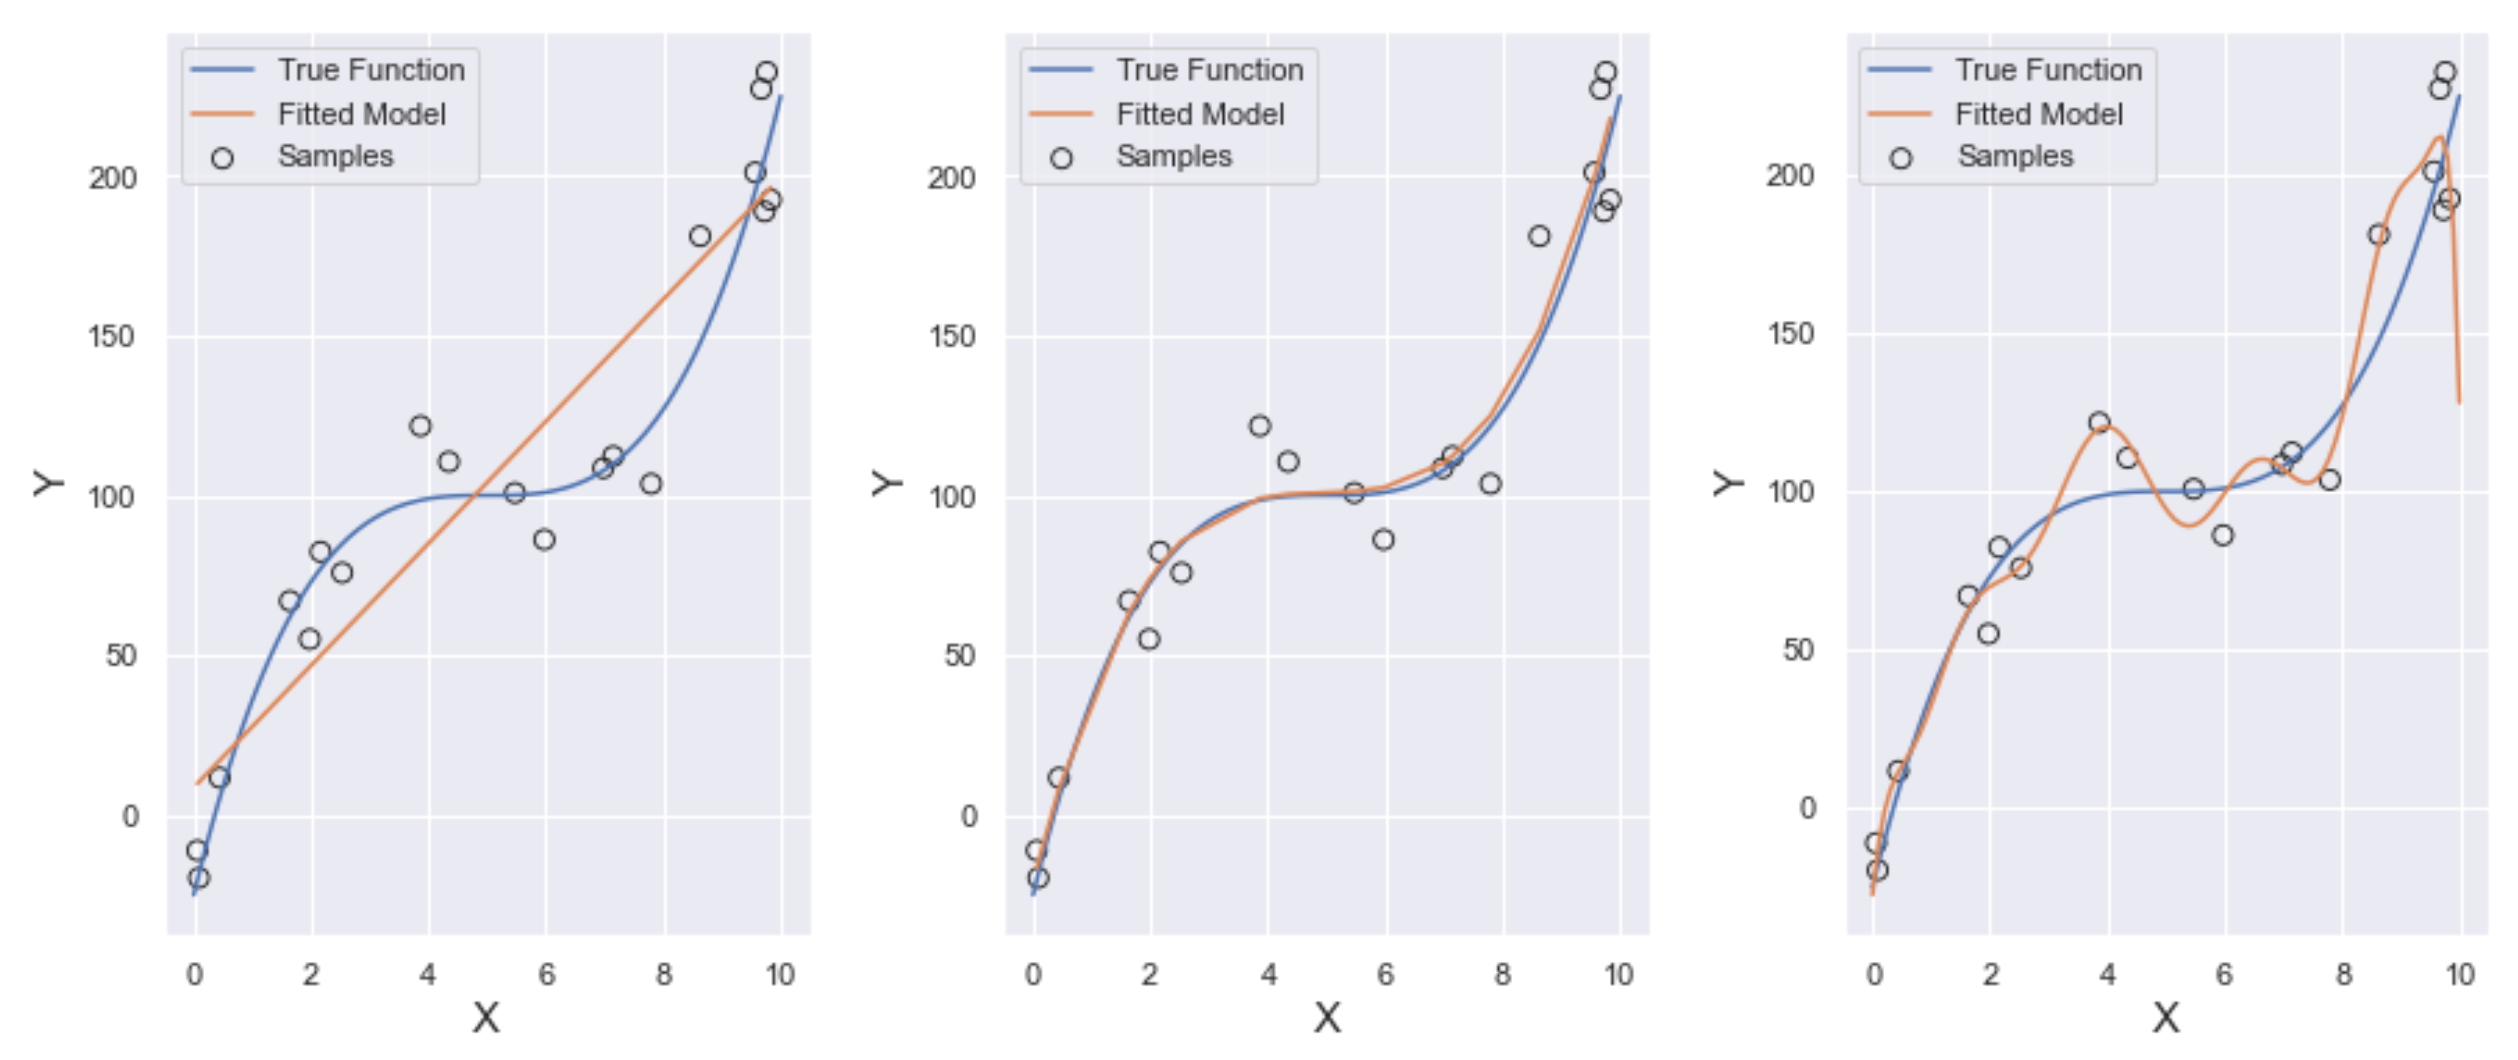
\includegraphics[scale=0.6]{Picture/overfit_underfit.png}


Fig: Underfitting (High bias low variance), Good fitting, and Overfitting (Low bias high variace)



\subsection{Subset Selection} 

\subsubsection{Best Subset Selection}

{\bf{Step 1}}: Let $\mathcal{M}_0$ be the base model with no feature such that the prediction is $y = \bar{y}$.

{\bf{Step 2}}: For $k = 1, 2, \cdots, p$ where $p$ is the total number of features in the data

\quad (A) Fit all $C(p, k)$ models $\{ \mathcal{M}_k^{(i)} \}$ 

\quad (B) From the set $\{ \mathcal{M}_k^{(i)} \}$ select the best model $\mathcal{M}_k$

{\bf{Step 3}}: Select best model from $\{ \mathcal{M}_0, \mathcal{M}_1, \cdots, \mathcal{M}_p \}$


\subsubsection{Forward Selection} 

{\bf{Step 1}}: Let $\mathcal{M}_0$ be the base model and initiate a feature set $\mathcal{F}_0 = \phi$ as a empty set.

{\bf{Step 2}}: For $k = 0, 1, \cdots, p-1$ where $p$ is the total number of features in the data

\quad (A) Fit all models $\{ \mathcal{M}_k^{(i)} \}$  such that $\mathcal{F}_k = \mathcal{F}_{k-1} \cup \{f_i \}$ where $i$ runs in remaining $p-k+1$ features.

\quad (B) From the set $\{ \mathcal{M}_k^{(i)} \}$ select the best model $\mathcal{M}_k$

{\bf{Step 3}}: Select best model from $\{ \mathcal{M}_0, \mathcal{M}_1, \cdots, \mathcal{M}_p \}$


\subsubsection{Backward selection }

{\bf{Step 1}}: Let $\mathcal{M}_p$ be the full model and $\mathcal{F}_p$ be a set of all features.

{\bf{Step 2}}: For $k = p, p-1, \cdots, 1$ 

\quad (A) Fit all models $\{ \mathcal{M}_k^{(i)} \}$  such that $\mathcal{F}_{k-1} = \mathcal{F}_k - \{f_i \}$ where $i$ runs in remaining $p-k$ features.

\quad (B) From the set $\{ \mathcal{M}_k^{(i)} \}$ select the best model $\mathcal{M}_k$

{\bf{Step 3}}: Select best model from $\{ \mathcal{M}_0, \mathcal{M}_1, \cdots, \mathcal{M}_p \}$


\subsection{$L_2$ Norm and Ridge Regression }



For the linear regression method $L_2$ regularization means adding $||\theta'||^2$ term to the cost function. 

$$
J(\Theta) = \epsilon^T \epsilon = (y - X\, \Theta)^T (y - X\, \Theta) + \lambda\, \theta^T\theta
$$

where $\lambda$ is the regularization parameter and  $\Theta = (\theta_0, \, \theta')$ indicating that we do not regularize the bias term. The close form solution exists for the linear regression 

$$
\Theta = (X^T X + \lambda I)^{-1} X^T y
$$

Usually a regression problem is over-determined system. Which means there are more equations than the variables. Simple regression method can not solve under-determined system though. However, Ridge regression can be used to solve the both under-determined and over-determined system. For the under-deterministic system, with  

$$A = (X, \sqrt{\lambda} \, I )^T \quad \text{and}\quad b = (y, 0)^T$$

we can also write the closed form solution as 

$$
\Theta = (A^T A)^{-1} A^T b 
$$

Hence $A$ is full rank even if $X$ is not a full rank matrix. Historically, ridge regression was introduced in this context. Now the update rule for the gradient descent changed to the following 

$$
\frac{\partial \, J(\Theta)}{\partial\, \Theta} = 2\, X^T (X\, \Theta - y) + 2 \lambda \, \theta
$$

Least square is scale invariant but regularized methods are not (May be this has to do with the fact that bias term is not regularized). Hence we use standardization before regularization methods. 



Alternatively we can write the porblem as a non-linear optimization problem as 

\begin{align*}
     \underset{x}{\mathrm{argmin}} \, & (y - X\, \Theta)^T (y - X\, \Theta) \\
    & \quad \theta^T\theta \leq t
\end{align*}

Where the first equation is the objective function and the second one is the constraint. The regularization term allocate a fixed budget for the coefficients. So they have to be wisely selected just to accommodate the important variables and giving small weight to the non-important variables. 





\subsection{$L_1$ Norm and Lasso Regression }


For the linear regression $L_1$ regularization means adding $||\theta'||$ term to the cost function. 

$$
J(\Theta) = \epsilon^T \epsilon = (y - X\, \Theta)^T (y - X\, \Theta) + \lambda ||\theta'||
$$

The closed form solution for Lasso does not exist even for the linear regression. This is because the $L_1$ penalty term is not differentiable and we can not use calculus to find the minimum loss unlike in Ridge regression. Even worse for the same reason we can not use the usual gradient descent algorithm either. There are some variations of gradient descent, like coordinate descent, sub-gradient descent etc. to solve this problem. For that reason Lasso is computationally more expensive than the Ridge regression. Alternatively we can pose this problem in terms of the linear optimization problem and solve from there.

\begin{align*}
     \underset{x}{\mathrm{argmin}} \, & (y - X\, \Theta)^T (y - X\, \Theta) \\
    & \quad ||\theta|| \leq t
\end{align*}


The difference between $L_1$ and $L_2$ normalization: $L_1$ norm shrinks the least important coefficient to zero to it can be used for the feature selector. However, $L_2$ norm only makes those terms very small and never shrinks to zero so it would be using all the features all the time. 






\newpage
\section{Model Selection}  


\subsection{Bias Variance Trade off }


Error in the testing data is 

$$
\delta = \hat{f}(x) - f(x) - \epsilon
$$

where $f(x)$ is the true function representing the relation of $x$ and $y$ such that $y = f(x) + \epsilon $ and $\hat{f}(x)$ our estimation of $f(x)$. Expectation (mean) of the squared error is 

$$
E\left[ \delta^2\right] = \left(\text{Bias}\left[\hat{f}(x)\right]\right)^2 + \text{Var}\left[\hat{f}(x)\right] + \sigma^2
$$

where $\sigma^2 = \text{Var}(\epsilon)$ is the variance of the random noise and is called irreducible error.  Bias and variance of the model $\hat{f}(x)$ are given by 

$$
\begin{align}
\text{Bias}(\hat{f}(x)) & = E[\hat{f}(x)]-f(x) \\
\text{Var}(\hat{f}(x)) & = E[\hat{f}(x)^2] - E[\hat{f}(x)]^2
\end{align}
$$

Bias means how much the model is representing the true relation between the variables. If we use a simple model it would have higher bias as it tend to be the oversimplified picture of the reality. On the other hand, variance means how much the model is stable if we use the different sample of training data from the same population. Simple model tend to be stable while more complex model tend to capture the noise of the data and varies a lot between sample to sample. Hence, there is a trade off between bias and variance. 

$$
\text{Simple Model = Low Bias + High Variance} 
$$
$$
\text{Complex Model = High Bias + Low Variance}
$$


\subsection{Estimating Prediction Error }

Parsimony principle: Choose the simpler model if its prediction error is similar to a more complex model. One simple way to estimate the prediction error is to divide the data into training, validation and testing error. Train data is used to train the data or learn the parameter of the model. Validation data is used to compare among different models and tune the hyperparameter of the model. Finally test data is used to predict the generalization error. For a smaller dataset it is not feasiable to split the data into train, validation, test sets. Hence we can use other analytical methods to access the model quality. The limitation of this methods is, however, many of the measures are not well defined for many black-box models and are available for few well understood models. 

For a linear model the parameter tuning is done using the following methods: 

$$
RSS = \sum_{i=1}^N (y-y_{pred})^2 
$$
$$
R^2 = 1 - \frac{RSS}{TSS}
$$

where $R^2$ is the estimation of the train set error. 

We can use following scores of estimate the test set error (without directly having test set):

$$
AIC = \frac{1}{N\hat{\sigma}^2}\left(RSS + 2 \hat{\sigma}^2 d\right) 
$$
$$
BIC = \frac{1}{N\hat{\sigma}^2}\left(RSS + \text{Log}(N) \hat{\sigma}^2 d\right)
$$
$$
C_p = \frac{1}{N}\left(RSS + 2 \hat{\sigma}^2 d\right
$$
$$
R^2_{adj} = 1 - \frac{RSS/(N-d-1)}{TSS/(N-1)}
$$


Where $d$ is the effective dimension of the model. All of them penaize for the large $d$ and can be used to tune the hyperparameter of the model. The limitation of this approach is that the effective dimension of not clearly known for all the models. 



\subsection{Cross-Validation Method }

Another simple approach to estimate the test error would be to divide the training data into two subsets, training set and testing set. It has two limitations: (1) Estimation of test error is highly variable among each possible splits. (2) Validation set error tend to overestimate the test set error compared to the model that would have fitted to the entire data. This is because the standard error varies inversely to the size of the training data and splitting reduces the size of the training data. However we can carefully look at the learning curve of the model. If the learning curve flats out at the size of the test data we are good to go. But if the learning curved is sloped at size of the test data we should look for the other alternative. 



Another extreme is to use leave one out cross validation (LOOCV). In this approach to can use all except one data point in training set and calculate the cross validation and repeat this process for leaving each data point for the validation one at a time and then averaging the cross-validation 

$$
CV_N = \frac{1}{N} \sum^N_{i=1} CV_i
$$


The main drawback of LOOCV is that it can be computationally very expansive if the data set is big.  On the other hand, the main benefits of LOOCV are (1) The cross-validation result is always the same as there is no randomness involved. (2) There is no overestimating of the training error as we are training on almost of same size of data as the original set. 

A balanced alternative approach is to use a cross-validation. In this approach we divide the data in $K$ roughly equal size partitions each of size $N_i, \, i = 1, 2, \cdots, K$. Take one of the partition as a validation set and rest together as training set. We then repeat the process for each partitions being validation set and take the average of the score 

$$
CV_K = \sum_{i=1}^K \frac{N_i}{N}\,  CV_i
$$

When each partitions are of equal size $N_i/N=K$ and hence we get a simple average. 



When we use large number of splits we use larger and larger set for training and the bias will be smaller and smaller in the model. But at the same time we are using smaller set for the validation and variance will go higher for the larger number of splits. On the other hand, if the number of split is smaller we are using smaller training set and bias will be higher. But the testing set is bigger and estimation has lower variance. So there is bias variance trade off involved in the optimal choice of $K$. Empirically, the optimal value of $K$ can be $5\leqslant K \leqslant 10$. LOOCV is the special case with $K=N$. 

One standard error rule in CV: In this approach we choose the most parsimonious model whose error is no more than one standard error above the error of the best model. 





\subsection{Bootstrap Methods }



Bootstrap is the sampling with replacement. Let $\hat{e}[\mathcal{S}^{(i)}]$ be an arbitrary statistics from a random sample $\mathcal{S}^{(i)}$, then with the bootstrap we can calculate the standard error of the statistics $\hat{e}$ as follows:

$$
SE[\hat{e}] = \frac{1}{n-1} \sum_{i=1}^n (\hat{e}[\mathcal{S^*}^{(i)}] - \bar{e}^*)^2
$$

where $\bar{e}^* =\sum_i \hat{e}[\mathcal{S^*}^{(i)}]/n$ is the mean of the sample mean and $\cal{S^*}$ is a bootstrap sample taken from the original sample $\cal{S}$. This method is also called Monte-Carlo estimation. 



For sample $\cal{S}$ of size $n$ the probability of its selection in a single draw is $1/n$ and not selecting it is thus $1-1/n$. Hence, if we draw a $n$ samples with replacement the probability of a particular data is not included in the final sample is for sufficuently large sample size 

$$
\lim_{n\to \infty} \left( 1 - \frac{1}{n} \right)^n = e^{-1} \approx 0.33
$$

Hence the expectation is roughly one third of the data will not show up in the final bootstrap sample. 



So here is the procedure: Take a bootstrap sample and fit the model. Calculate the test error on the $33\%$ of the data not appeared on the bootstrap. Keep repeating this sufficiently large number of times. The average of the test error gives the estimate of the test error and on bonus we can also calculate the standard error of the test error. One of the main drawback of bootstrap method is that it has set train test split of ratio $2:1$. Which might not be the ideal case for a small data. 



\newpage
\section{Decision Tree}

\subsection{Regression Tree }

Regression tree makes a binary split into the data such that 

$$
\mathcal{R}_1 (j, s) = \{x | x_j < s\} \quad \text{and} \quad \mathcal{R}_2 (j, s) = \{x | x_j \geq s \}
$$


where $s$ is a carefully chosen threshold optimizing the cost function. The cost function is given by 

$$
\min_{j,\, s} \left[ \min_{c_1} \sum_{x_j \in \mathcal{R}_1} (y_j - c_1)^2 +  \min_{c_2} \sum_{x_j \in \mathcal{R}_2} (y_j - c_2)^2 \right]
$$

where the impurity measure of the region $\cal{R}$ with a predefined constant $c_\cal{R}$ is a for the region is defined as 

$$
I(j, \mathcal{R}) = \sum_{x_j \in \mathcal{R}} (y_j - c_\mathcal{R})^2 
$$


The inner minimization be achieved if $c_1$ and $c_2$ are given by the averages $\hat{y}_{\mathcal{R}_1}$ and $\hat{y}_{\mathcal{R}_2}$ in their respective split. Hence the cost function is 

$$
\min_{j,\, s} \left[ \sum_{x_j \in \mathcal{R}_1} \left(y_j - \hat{y}_{\mathcal{R}_1} \right)^2 + \sum_{x_j \in \mathcal{R}_2} \left(y_j -  \hat{y}_{\mathcal{R}_2} \right)^2 \right]
$$

Larger tree can easily overfit the training data. Hence, tree pruning is needed. There are many ways to prune a tree, for example: limiting tree depth, limiting total number of leaves, limiting total number of splits etc. One of the way to regularize the tree growth is by adding a penalty in the cost function 

$$
\min_{j,\, s} \left[\,\, \sum_{m=1}^{n(T)} \, \, \sum_{x_i \in \mathcal{R}_m} \left(y_i - \hat{y}_{\mathcal{R}_m}\right)^2 + \alpha \, n(T) \right]
$$

where  $n(T)$ is the number of terminal (leaf) nodes in the tree and $\alpha$ is the regularization parameter. The outer sum spans over all the leaf nodes and the inner sum spans over all the data in a particular leaf node. The trees pays higher price is the tree is large with high $n(T)$. However, there are other methods too to regularize tree such as directly controlling the number of leaves, tree depth, minimum data in a leaf, minimum data to make a split, minimum information gain to make a split etc. Despite of all these tools decision tree is prone to overfit the training data.



\subsection{Classification Tree }

If the feature variable is continious and only the target is discrete then the classification tree is similar to the regression tree expect the impurity measure is either entropy or Gini index. 

$$
\text{Gini Index} = \sum_{k=1}^K \hat{p}_{mk} (1 - \hat{p}_{mk})
$$
$$
\text{Entropy} = - \sum_{k=1}^K \hat{p}_{mk}\, \text{log}\,\hat{p}_{mk} 
$$

where $\hat{p}_{mk}$ is the probability of a data from $m^{th}$ region belong to $k^{th}$ category and is given by counting the frequency of the category in the given class

$$
\hat{p}_{mk} =\frac{1}{N_m} \sum_{x_i \in \mathcal{R}_m} I (y_i = k)
$$

Hence, with Gini index and entropy, the regularized cost function is given respectively by 

$$
\min_{j,\, s} \left[\,\, \sum_{m=1}^{n(T)} \, \, \sum_{k=1}^K \hat{p}_{mk} (1 - \hat{p}_{mk}) + \alpha \, n(T) \right]
$$

$$
\min_{j,\, s} \left[\,\, \sum_{m=1}^{n(T)} \, \, \sum_{k=1}^K \hat{p}_{mk}\, \text{log}\,\hat{p}_{mk}  + \alpha \, n(T) \right]
$$

where the second term is regularization term as usual.  



\subsection{Categorical Features }


With the categorical variable $x | x \in \mathcal{G} = \{\mathcal{C}_1, \mathcal{C}_2, ... \mathcal{C}_q\}$ the split between the two regions look like this 

$$
\mathcal{R}_1 (j, s) = \{x | x_j \in {\cal{G}}_1\} \quad \text{and} \quad \mathcal{R}_2 (j, s) = \{x | x_j \in {\cal{G}}_2 \}
$$

where $\mathcal{G}_1$ and $\mathcal{G}_2$ are two two disjoint subset of $\mathcal{G}$ such that $\mathcal{G}_1 \cup \mathcal{G}_2 = \mathcal{G}$. The subsets are carefully chosen to minimize the impurity. Unlike the numerical feature, there is no sense of ordinality in the cardinal features and hence we need to check all possible splits between  $\mathcal{G}_1$ and $\mathcal{G}_2$ which totals $2^{q-1}-1$ possible combinations. Hence, for high cardinality categorical feature this calculation can be costlier. 


\subsection{Python Implementation}

Implement regression and classification tree classes 





\newpage
\section{Additive Models \& Ensembles}

\subsection{Generalized Additive Model }

Find a good place to put this

Generalized additive models are a way to generate non-linear fit 

$$
y = \alpha + \sum_{j=1}^p f_j(X_j) + \epsilon
$$

The cost function is 


$$
\sum_{i=1}^N \left( y_i - \alpha - \sum_{j=1}^p f_j(x_{ij}) \right)^2 + \sum_{j=1}^p \lambda_j \int [f''_j (t_j)]^2 dt_j
$$


where the second term is the regularization term without it $f(x)$ will simply interpolate between all the data points and overfit the data. $f''(x)$ is the measure of the curvature and a wigly curve will pay higher price for having high curvature everywhere and model tries to find less wigly curve. 



Unbalanced data 

\subsection{Random Forest }


{\bf{Step 1}}: For $m = 1, 2, ..., M$:

\quad	(A) Randomly select $q = \sqrt{p}$ features from the total $p$ features 

\quad	(B) Use bootstrap sampling to create a sample $\cal{S}^*$ of size $N$ with $q$ selected features. 

\quad	(C) Grow a desicision tree on $\cal{S}^*$. 

{\bf{Step 2}}:  Make a final decision with the vote of $M$ decision trees. 


\subsection{Gradient Boosting }

For data $\{(x_i, y_i)\}$ and a differentiable loss function $L(y_i, F(x))$

{\bf{Step 1}}:  Initialize the model with a constant value $F_0(x) = \underset{\gamma}{\mathrm{argmin}} \sum_{i=1}^N L(y_i, \gamma)$. 

{\bf{Step 2}}:  for $m=1, 2, ... , M$:

\quad	(A) Compute $r_{im} = -\left[\frac{\partial L(y_i, F(x_i))}{\partial F(x_i)} \right]_{F(x) = F_{m-1}(x)}$ for $i = 1, 2, ..., n$. 

\quad	(B) Fit a regression tree to the $r_{im}$ values and create terminal region $\mathcal{R}_{jm}$ for $j = 1, 2, ..., J_m$. 

\quad	(C) For $j = 1, 2, ..., J_m$ compute $\gamma_{im} = \underset{\gamma}{\mathrm{argmin}} \sum_{x_i \in \mathcal{R}_{ij}} L(y_i, F_{m-1}(x_i)+ \gamma )$ . 

\quad	(D) Update $F_m(x) = F_{m-1}(x) + \nu \sum_{j=1}^{J_m} \gamma_{jm} I(x \in \mathcal{R}_{jm})$. 

{\bf{Step 3}}:  Output $F_M(x)$. 


\subsection{XGBoost, LightGBM \& Catboost }



% \newpage
% \section{Neural Network}

% \subsection{Feed Forward Neural Network}

% \subsection{Back-propagation }

% \subsection{Training a Neural Network }


% \subsection{Convolutional Neural Network }

% \subsection{Sequence Model }



\newpage
\section{Support Vector Machine}



\subsection{Polynomial Features }



Consider the polynomial regression 

$$
y = \theta_0 + \theta_1 x + \theta_2 x^2 + \theta_3 x^3 = \Theta^T\phi(x)
$$

where $\phi(x) = (1, x, x^2, x^3)^T$.  Then the corresponding cost function is 

$$
J(\Theta) = \frac{1}{2N} \sum_{i=1}^N \left(y^{(i)} - \Theta^T\phi(x^{(i)})\right)^2
$$

Then the update rule for the gradient algorithm is 

$$
\Theta := \Theta + \frac{\alpha}{N} \sum_{i=1}^N \left(y^{(i)} - \Theta^T\phi(x^{(i)})\right)\phi(x^{(i)})
$$


\subsection{Kernels }



The set of polynomials $\phi(x)$ acts as a basis set in the feature space. As a result we can write any vector including $\Theta$ as a linear combination of those. 


$$
\Theta = \sum_{i=1}^N \alpha_i \, \phi(x^{(i)})
$$


Hence the predicted value is  

$$
y = \Theta^T \phi(x) = \sum_{j=1}^N \alpha_j \, \phi(x^{(j)})\phi(x) = \sum_{i=1}^N \alpha_i K(x^{(i)}, x)
$$


where $K(x^{(i)}, x) = \sum_j \phi(x_j^{(j)})\phi(x_j)= \langle \phi(x^{(i)})\phi(x) \rangle$ is called kernel and is an inner product of the feature vector.  The cost function in terms of kernel is then 


$$
J(\Theta) = \frac{1}{2N} \sum_{i=1}^N \sum_{j=1}^N \left(y^{(i)} - \alpha_i K(x^{(i)}, x^{(j)})\right)^2
$$


The update rule can be written in terms of the kernel as well. First write this as 

$$
\Theta := \sum_{i=1}^N \alpha_i \, \phi(x^{(i)}) + \frac{\alpha}{N} \sum_{i=1}^N \left(y^{(i)} - \Theta^T\phi(x^{(i)})\right)\phi(x^{(i)})
$$

where we only replace first $\Theta$ by the basis expansion while the second $\Theta$ inside the summation is untouched. Next we factor out the basis inside the summation. 

$$
\Theta := \sum_{i=1}^N \left[\alpha_i + \frac{\alpha}{N} \left(y^{(i)} - \Theta^T\phi(x^{(i)})\right)\right]\phi(x^{(i)})
$$


Now the expansion coefficient $\alpha_i + \frac{\alpha}{N} \left(y^{(i)} - \Theta^T\phi(x^{(i)})\right)$ can be written in terms of the kernel. 


$$
\alpha_i := \alpha_i + \frac{\alpha}{N} \left(y^{(i)} - \sum_{j=1}^N \alpha_j K(x^{(i)}, x^{(j)})\right)
$$


Hence we first update $\alpha_i$ and then update $\Theta$ consequently. 


\subsection{Kernel Trick }

How mapping in a higher dimension helps?


\subsection{Separating Hyperplane }

Let $x_i^T\alpha + \alpha_0$ is the separating hyperplane such that 

$$
\begin{align}\nonumber
& x_i^T\alpha + \alpha_0 > 0 \qquad\qquad \text{for}\quad y_i = +1 \\ 
& x_i^T\alpha + \alpha_0 < 0 \qquad\qquad \text{for}\quad y_i = -1 
\end{align}
$$


Combining both $y_i(x_i^T\alpha + \alpha_0)>0$ is the separating hyperplane for both the cases.  Geometrically, $y_i(x_i^T\alpha + \alpha_0)>0$  is the projection of the data point onto the separating hyperplane, which in turn is the distance of each of the data point from the separating hyperplane. We are interested to find the maximum margin classifier which maximize the margin $M$ between the two classes from the separating hyperplane. 


$$
\begin{align}\nonumber
& \max_{\alpha_0, \alpha_1, \cdots, \alpha_p} M  \\ \nonumber
 y_i & (x_i^T\alpha + \alpha_0) \geqslant M \\
& \sum_{i=1}^p \alpha_i^2 = 1
\end{align}
$$


where $i = 1, 2, \cdots, N$. First condition requires the margin to be maximize. The second condition requires that all the observation points are on the correct side of the hyperplane and are at least $M$ distance away from the hyperplane. What the last condition means the orientation of the separating hyperplane is characterized by a unit vector and the intercept term $\alpha_0$ is not constrained by this condition as it should be. 



Below we discuss Non-Separable Case / Support Vector Classifier. Here we generalize the idea of the separating hyperplane to address two of its shortcomings: (1) data may be linearly inseparable still having optimal linear decision boundary, (2) The data can be noisy and a single outlier may drastically change the separating hyperplane. Hence we introduce the idea of soft margin in which we allow few of the observation to lie on (A) the wrong side of the margin and/or (B) the wrong side of the hyperplane. 


$$
\begin{align}\nonumber
 & \qquad \max_{\alpha_0, \alpha_1, \cdots, \alpha_p} M  \\\nonumber
 y_i & (x_i^T\alpha + \alpha_0) \geqslant M(1-\zeta_i)  \\
\zeta_i \geqslant 0, & \quad \sum_{i=1}^N \zeta_i \geqslant C, \quad \sum_{i=1}^p \alpha_i = 1
\end{align}
$$


- $\zeta_i$ are called slack variables. An observation point is in the right side of the margin, wrong side of the margin and wrong side of the hyperplane depending on whether $\zeta_i = 0$ , $\zeta_i > 0$ and $\zeta_i > 1$. This is the origin of hinge loss function of SVM classifier.  

- $C$ controls the regularization of the model. Larger $C$ allows more points on the wrong side while small $C$ restricts more points to be on the right side. In particular $C=0$ requires $\zeta_i = 0$ for all the observation points. Hence larger $C$ means high bias and low variance while on the other hand smaller $C$ means low bias and high variance.  
- In this method only those observation on the wrong side of the margin or on the margin affect the location of decision boundary. These observation points are called support vectors. When $C$ is large, there are more support vectors and when $C$ is small, there are less support vectors. 
- We can combine $C$ term with the objective function making it a Lagrange multiplier $M + C \sum_{i=1}^N \zeta_i$. This is called hinge loss function. 



\subsection{Non-Linear Boundary / Support Vector Machine }



Separating hyperplane method generalized for non-separable hyperplane which is further generalized for non-linear boundary typically handled with method of kernel is called Support Vector Machine classifier. The separating hyperplane is 

$$
f(x) = \alpha_0 + \sum_{i\in \mathcal{S}} \alpha_i K(x, x_i)
$$

Generally the summation is taken over all the observations $N$. However, in practice we do not have to sum over all the observation but only subset of observations which belong to the support vectors $\mathcal{S}$. The choice of linear kernel gives the linear boundary. We can choose non-linear kernel for the non-linear boundary. 

$$
\begin{align}
\text{Linear} \qquad & K(x, x') = \langle x, x' \rangle \\
\text{Polynomial} \qquad   & K(x, x') = (1+\langle x, x' \rangle)^d\\
\text{Radial Basis} \qquad	& K(x, x') = \text{e}^{-\gamma||x-x'||^2}
\end{align}
$$


Alternatively the support vector machine cost function can be expresses as 
$$
J(\Theta) = \sum_{i=1}^N \text{max}\left(0, 1 - y_i f(x_i)\right) + \lambda \sum_{j=1}^p \alpha_j^2
$$


In this form the cost function = loss + penalty. The loss function is called hinge loss function. The regularization coefficient $\lambda$ is directly related to the coefficient $C$ earlier. 



\newpage
\section{Generative Models}

\subsection{Discriminateive Models vs Generative}

\subsection{Naïve Bayes }

Bayes theorem states that

$$
p(C_k|X) = \frac{p(X|C_k) \, p(C_k)}{p(X)}
$$


Denominator is same for all and we can ignore it. Now, we make a "naïve" assumption that all the features are independent to one another. This assumption might not be true and might affect the value of exact probability. But we are comparing probability of one class vs other in order to make a classification. So, this method work just fine. 

$$
p(C_k|X) = p(C_k) \prod_{i=1}^M p(X_i |C_k)
$$

Naïve bias can handle multicollinearity or even more extreme it is possible that $X_i=X_j$ for $i\neq j$ and naïve bias still works fine. If $p(X|C)$ are calculated using the Gaussian distribution then it is called the Gaussian naïve bias. Otherwise, we can estimate them by using histogram of the observed data. In this case it is called the multinomial naïve bias. Since, we would be most likely multiplying small numbers, it is numerically efficient to take the logarithm to avoid "underflow problem". 
$$
\text{Log}\left( p(C_k | X) \right) = \text{Log}\left( p(C_k)\right) + \sum_{i=1}^M \text{Log}\left(p(X_i|C_k)\right)
$$


The first term on the right hand side is called prior. With zero correction 

$$
\text{Log}\left( p(C_k | X) \right) = \text{Log}\left( p(C_k)\right) + \sum_{i=1}^M \text{Log}\left(p(X_i|C_k)+ \alpha \right)
$$

Naïve bias is naïve because it does not care the word order and treats the language as bag of words. 





\subsection{Linear Discriminant Analysis }

We can start with the Bayes rule for the case of distribution function 

$$
p(y=i|X) = \frac{f_i(x)\, \pi_i}{\sum_{j=1}^K f_j(x)\pi_j}
$$


where $\pi_i$ is the prior probabilities. Now log of the odds are given by 
$$
\text{Log}\, \frac{p(y=i|X)}{p(y=j|X)} = \text{Log}\,\frac{\pi_i}{\pi_j} + \text{Log}\,\frac{f_i(x)}{f_j(x)}
$$


Discriminant analysis is more restrictive because we need to make an assumption about the distribution of the data $f(x)$. For many case we can assume that the distribution is normal. Following is the expression for the multinomial normal distribution

$$
f_i(x) = \frac{1}{(2\pi)^{p/2}{\bf{\Sigma}}_i^{1/2}} e^{-\frac{1}{2}(x-\mu_i){\bf{\Sigma}}_i (x-\mu_i)}
$$


where $\bf{\Sigma}$ is the covariance matrix whose diagonal elements are the variances and $p$ is the dimension of the distribution. With the assumption that ${\bf{\Sigma}}_i = {\bf{\Sigma}} \, \forall i$, then log of the odds simplifies to 

$$
\delta_i(x) = \text{Log}\, \pi_i - \frac{1}{2}\mu_i^T{\bf{\Sigma}}^{-1}\mu_i + x^T{\bf{\Sigma}}^{-1}\mu_i
$$

This gives us a linear decision boundary. 



\subsubsection{QDA}

If we don't make the assumption that ${\bf{\Sigma}}_i = {\bf{\Sigma}} \, \forall i$, the we get 

$$
\delta_i(x) = \text{Log}\pi_i -\frac12 \text{Log} |{\bf{\Sigma}}_i| - \frac12 (x-\mu_i)^T {\bf{\Sigma}}_i^{-1} (x-\mu_i) 
$$

Hence the decision boudnary is quadaratic in this case. 





\subsection{Gaussian Mixture Model }



\newpage
\section{Prototype Models}

\subsection{k-Nearest Neighbor}


Lazy and eager methods 

\subsection{Python Implementation of KNN}


\subsection{k-Mean Clustering }

{\bf{Step 1}}: For data $\{x_i\} \in \mathbb{R}^N$ initialize $K$ centroids $\{\mu_1, \mu_2, ..., \mu_K\} \in \mathbb{R}^N$ randomly. 

{\bf{Step 2}}: Repeat the following until convergence:

\quad		(A) For $i = 1, 2, ..., N$ set $c^{(i)} = \underset{j}{\mathrm{argmin}} \left[D(x^{(i)}, \mu_j)\right]$ such that $x^{(i)}\in \mathcal{R}_j$. 

\quad		(B) For $j = 1, 2, ..., K$ set $\mu_j = \frac{\sum_{i\in \mathcal{R}_j} \mathbb{I}\{c^{(i)}=j\} \, x^{(i)}}{\sum_{i\in \mathcal{R}_j} \mathbb{I}\{c^{(i)}=j\}}$. 

{\bf{Step 3}}: Return the set $\{x^{(i)}\}\in \mathcal{R}_j,  \, \forall j = 1, 2, ..., K$. 



Where $D(x^{(i)}, \mu_j)$ is distance matrix and a few common choice of distance matrix are following 

$$
\text{Euclidean:} \qquad D(x^{(i)}, \mu_j) = \sum_i (x^{(i)} - \mu_j)^2 
$$
$$
\text{Manhattan:} \qquad D(x^{(i)}, \mu_j) = \sum_i |x^{(i)} - \mu_j|
$$


 The cost function of the problem is the within-point scatter and is given by 
 
$$
W(x^{(i)}, \mu_j) = \sum_{j=1}^K \sum_{i\in \mathcal{R}_j}  D(x^{(i)}, \mu_j)
$$


This is the sum of distance of each data points from the centroid of their assigned cluster and can be thought as a cost function. This is a non-convex optimization problem and hence the algorithm can end in a bad local optima. For that reason it is advised to repeat the algorithm with few different random initialization and take the set $\{\mathcal{R}_j\}$ that minimize $W(x^{(i)}, \mu_j)$ for given $K$. The optimal number of clusters $K$ is chosen such that $W(x^{(i)}, \mu_j) $ is minimized. 

\subsection{Python Implementation of KMC}

\subsection{Hierarchical Clustering }


\newpage
\section{Factor Analysis}

\subsection{Principle Component Analysis }

Let $X = \{x_{ij}\}, \, i = 1, 2, ..., N \, \text{and}\, j = 1, 2, ..., p $ be a matrix representing the data where $N$ is the number of observations and $p$ is the number of features. Let us assume that each features are centered around zero and have unit variance. If not we can make the following transformation 

$$
x_{ij} = \frac{x_{ij} - \bar{x}_j}{\sigma_{j}}
$$

Now let $U = \{ u_{ij} \}$ be a $p\times p$ matrix with $p$ number of $p$ dimensional basis vectors $u_j$ on the columns. Then we can transform the original feature matrix $X$ by $U$ such that $P= X U$ to optimize 

$$
 P^T P = (X U)^T (X U) = U^T (X^T X) U = U^T D \, U
$$

Where $D = X^T X$ is identified as the covariance matrix among different feature and has a dimension $p\times p$. The optimimum value of the equation is provided by the eigen vector of $D$ when $U$ is orthogonal. In that case $D$ is a diagonal matrix with diagonal elements being the eigenvalue of $P^T P$ and the columns of $U$ are the corresponding eigenvectors. Hence, the above equation is identified as a principal value decomposition. The first principal vector is the eigen vector with the maximum eigen value and gives the direction of the maximum variance in the data. The second principal component is the eigen vector with the second highest eigen value and gives the direction of the second highest variance which is orthogonal to the hyperplane defined by the earlier principal components and so on. 



Alternatively the PCA can be calculated from the singular value decomposition of the feature matrix $X$ directly. 

$$
X = M D N^T
$$

How the two approaches are related?



PCA can be used for dimensionality reduction. 


\subsection{Independent Component Analysis}


\subsection{Singular Value Decomposition}





\newpage
\section{Homeworks}


\subsection*{Student Learning Outcomes (SLO)}

By the end of this course the students will be able to 
\begin{enumerate}
    \item Understand the mathematical concept behind the major machine learning algorithms. 
    
    \item Implement the major machine learning algorithms in python using object oriented design 
    
    \item Read and understand the documentation of major machine learning library 
    
    \item Read and understand the source code of major machine learning library
    
    \item Solve the real life problem with their own implementation and/or standard machine learning library 
\end{enumerate}

\newpage

\subsection*{Homework 1}


\begin{enumerate}
    \item In the normal equation of the linear regression $\hat{\Theta} = (X^T X)^{-1} X^T y$ the part $(X^T X)^{-1} X^T$ is called the pseudo-inverse of the matrix $X$. Show that the pseudo-inverse reduce to the inverse of the matrix $X$ if it is a square matrix. 
    
    \item The update rule for the gradient descent for the linear regression is given by 
    $$\Theta =  \Theta -  2\,\alpha \, X^T (X\, \Theta - y) $$
    Show that we can separate the weights and bias part and write the update rule as follows 
    $$ W = W -  2\,\alpha \, X^T (X\cdot W + b - y)  $$
    $$ b =  b -  2\,\alpha \, \sum_i (x_i \, w_i + b - y_i) $$
    
    \item Modify the python implementation of the linear regression in the text such that the gradients are updated with stochastic gradient descent.
    
    \item Use your implementation in the above equation to predict the Boston house price. 
    
    \item Starting with 
    $$
    \text{Log}\left(\frac{p(y=0|X)}{p(y= 1|X)}\right) = X \Theta + \epsilon
    $$
    show that 
    $$
    p(y=0|X) = \frac{1}{1 + e^{-z}}
    $$
    where $z= X \, \Theta + \epsilon $
    
    \item Derive the update rule for the Logistic regression 
    
    \item Modify the Logistic regression implementation in the text for the multi-class classification problem using soft-max regression. 
    
    \item Use the implementation above to classify Iris flower 
    
\end{enumerate}




$$
Y_t = \nabla^d X_t = (1 - B)^d X_t \quad \text{s.t.}\quad Y_t \sim N(\mu, \sigma^2)
$$


$$
\rho(X_t,\, X_{t-i})  \begin{cases}
      > 0 & \text{if $i = n s$,   $n \in \mathbb{Z^{+}}$}\\
      = 0 & \text{else}
    \end{cases} 
$$


$$

$$



\end{document}